\documentclass[article,10pt,a4,oneside]{memoir}
\usepackage[danish]{babel}
\usepackage[T1]{fontenc}
\usepackage[utf8]{inputenc}

\usepackage{amsmath}%
\usepackage{amsfonts}%
\usepackage{amssymb}%
\usepackage{graphicx}
%\usepackage[hmargin=3cm,vmargin=0.5cm]{geometry}
\usepackage{color}
\usepackage{caption}
\usepackage{tikz}

\pagestyle{empty}
\setlrmarginsandblock{1cm}{1cm}{*}
\setulmarginsandblock{1.2cm}{1.2cm}{*}
\checkandfixthelayout[nearest]

%Dagens datalog
%Madandmeldelse: DSB-kaffe
%Parring: Ewok
%Vejr: Aarhus 100 år
\begin{document}
\title{UNF Matematikcamp 2013 \\ Dagseddel søndag}

\begin{minipage}[b]{0.95\textwidth}
\fcolorbox{black}{white}{
\begin{minipage}[b]{0.2\linewidth}

\includegraphics[width=0.5\linewidth]{unflogo.pdf}
\end{minipage}
\begin{minipage}[b]{0.35\linewidth}
\Huge \textbf{UNF NEWS} \\
\Large -- Jyllands største avis
\end{minipage}
\begin{minipage}[b]{0.4\linewidth}
\Large Søndag 13.07.2012 \\
\normalsize Redigeret i \LaTeX\ af \\

\end{minipage}
}
\end{minipage}

\begin{minipage}[b]{0.95\textwidth}
\begin{minipage}[t]{0.47\textwidth}
\vspace{3mm}

\section*{Velkomst}
Kære deltagere,

I har nu begivet jer på en rejse mod solopgangen, i håbet om at finde frelsen i matematik. Frygt ikke, I er kommet det rette sted, fra her er der kun to veje, lysets og mørkets. Lysets vej er nemmest, men anvendt frem for dyb, det er fysikerens og datalogens forfejlede retning, fyldt med usikkerheder og manglende forståelse for den ægte sandhed. Her er vi på vejen mod mørket, omgivet af mangfoldigheder og indlejret i rum, hvis indre produkt sandeligt er positiv og definit.

Det var i herrens år 2007, da barbariet endte og mennesket blev sig selv bevidst. En mørk sommeraften mødtes forskrækkede matematikere ved Odins vig for at aksiomatisere livet og verden. Sidenhen, hver gang året står på sit højeste, mødes de, sidenhen skiftende steder på den jydske hede og på mons Hafniae.

Svensken truer mod øst, og Jyden truer mod vest, men dette skal ikke bekymre jer endnu, angsten kan vente til mandag. Fryd jer, mød hinanden, lær og læs og dø kun når I har fået lov. 

{\flushright\emph{Jeres koordinator, Helene}}

\section*{Velkomst}
Kære deltagere,

I har nu begivet jer på en rejse mod solopgangen, i håbet om at finde frelsen i matematik. Frygt ikke, I er kommet det rette sted, fra her er der kun to veje, lysets og mørkets. Lysets vej er nemmest, men anvendt frem for dyb, det er fysikerens og datalogens forfejlede retning, fyldt med usikkerheder og manglende forståelse for den ægte sandhed. Her er vi på vejen mod mørket, omgivet af mangfoldigheder og indlejret i rum, hvis indre produkt sandeligt er positiv og definit.

Det var i herrens år 2007, da barbariet endte og mennesket blev sig selv bevidst. En mørk sommeraften mødtes forskrækkede matematikere ved Odins vig for at aksiomatisere livet og verden. Sidenhen, hver gang året står på sit højeste, mødes de, sidenhen skiftende steder på den jydske hede og på mons Hafniae.

Svensken truer mod øst, og Jyden truer mod vest, men dette skal ikke bekymre jer endnu, angsten kan vente til mandag. Fryd jer, mød hinanden, lær og læs og dø kun når I har fået lov. 

{\flushright\emph{Jeres koordinator, Morten Agger}}

\end{minipage}
\hfill\begin{minipage}[t]{0.47\textwidth}

\vspace{1mm}
\tikzstyle{mybox} = [draw=white, fill=blue!20, very thick,
    rectangle, rounded corners, inner sep=10pt, inner ysep=20pt]
\tikzstyle{fancytitle} =[fill=red, text=white]

\begin{tikzpicture}
\node [mybox] (box){%
\begin{minipage}{0.80\textwidth}
\vspace{-4mm}\section*{Dagens program}
\begin{tabular}{ll}
12:00-13:00 & Ankomst \\
13:00-14:00 & Frokost \\
14:00-16:00 & Sociale arrangementer \\
16:00-16:30 & Faglig introduktion \\
16:30-18:00 & Sociale arrangementer \\
18:00-19:00 & Middag \\
19:00-21:00 & Sociale arrangementer \\
\end{tabular}
\vspace{-4mm}
\end{minipage}
};
\end{tikzpicture}%

\section*{Velkomst}
Kære deltagere,

I har nu begivet jer på en rejse mod solopgangen, i håbet om at finde frelsen i matematik. Frygt ikke, I er kommet det rette sted, fra her er der kun to veje, lysets og mørkets. Lysets vej er nemmest, men anvendt frem for dyb, det er fysikerens og datalogens forfejlede retning, fyldt med usikkerheder og manglende forståelse for den ægte sandhed. Her er vi på vejen mod mørket, omgivet af mangfoldigheder og indlejret i rum, hvis indre produkt sandeligt er positiv og definit.

Det var i herrens år 2007, da barbariet endte og mennesket blev sig selv bevidst. En mørk sommeraften mødtes forskrækkede matematikere ved Odins vig for at aksiomatisere livet og verden. Sidenhen, hver gang året står på sit højeste, mødes de, sidenhen skiftende steder på den jydske hede og på mons Hafniae.

Svensken truer mod øst, og Jyden truer mod vest, men dette skal ikke bekymre jer endnu, angsten kan vente til mandag. Fryd jer, mød hinanden, lær og læs og dø kun når I har fået lov.
 
{\flushright\emph{Jeres koordinator, Morten Grue Sørensen}}

\end{minipage}
\end{minipage}













\eject \pdfpagewidth=420mm \pdfpageheight=297mm
\begin{minipage}[b]{1.95\textwidth}
\begin{minipage}[t]{0.48\linewidth}
\fcolorbox{black}{white}{
\begin{minipage}[b]{0.2\linewidth}

\includegraphics[width=0.5\linewidth]{unflogo.pdf}
\end{minipage}
\begin{minipage}[b]{0.35\linewidth}
\Huge \textbf{UNF NEWS} \\
\Large -- Jyllands største avis
\end{minipage}
\begin{minipage}[b]{0.4\linewidth}
\Large Søndag 13.07.2012 \\
\normalsize Redigeret i \LaTeX\ af \\

\end{minipage}
}
\end{minipage}
\hfill
\begin{minipage}[t]{0.48\linewidth}
\fcolorbox{black}{white}{
\begin{minipage}[b]{0.2\linewidth}

\includegraphics[width=0.5\linewidth]{unflogo.pdf}
\end{minipage}
\begin{minipage}[b]{0.35\linewidth}
\Huge \textbf{UNF NEWS} \\
\Large -- Jyllands største avis
\end{minipage}
\begin{minipage}[b]{0.4\linewidth}
\Large Søndag 13.07.2012 \\
\normalsize Redigeret i \LaTeX\ af \\

\end{minipage}
}
\end{minipage}
\end{minipage}

\begin{minipage}[b]{1.95\textwidth}
\begin{minipage}[t]{0.23\linewidth}
\vspace{3mm}
\section*{Parringsritual -- Ewok}

\begin{center}
%$\quad$\hspace{4cm}
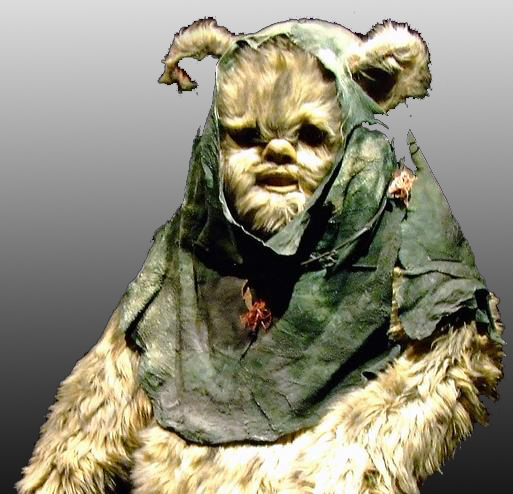
\includegraphics[width=0.8\linewidth]{Ewok.jpg}
\end{center}
\end{minipage}
\hspace{2mm}
\begin{minipage}[t]{0.46\linewidth}
%\vspace{3mm}



\begin{center}
\includegraphics[width=0.7\linewidth]{TooManyPigeons.jpg}
%\captionof*{figure}{\hspace{3cm}Dueslagsprincippet\\ \vspace{1mm} \\ \tiny en:User:BenFrantzDale og en:User:McKay, CC-BY-SA 3.0}
\end{center}
\end{minipage}
\hspace{2mm}
\begin{minipage}[t]{0.23\linewidth}

\vspace{1mm}

\section*{Madandmeldelse -- DSB-kaffe}
Det ses ved første øjenkast at her er der virkelig kræset for detaljerne, udstyr til kropslig styrkelse er blandet med mentale udfordringer i symmetrisk placerede badefaciliteter og kunstnerisk udførte lysinstallationer, som spiller godt sammen med den historicistiske hovedbygning fra 1890'erne. Også for det fysiske velvære er sørget, velvidende at frost hyppigt kan forekomme i den danske sommer, så der er sørget for den nødvendige mængde kropsvarme i lokalet, og af miljøhensyn desuden sparet på udluftningen.
Endda lydbilledet er proffesionelt konstrueret, med en passende mængde af snorken, luftmadrasser der sprænges klokken tre og en decent men veliscenesat piplyd fra et ukendt sted. Gadelarmen understreger rummets urbane placering på Indre Østerbro og sirener minder jævnligt om Rigets betryggende nærhed. Hvis vinden kommer fra den rigtige retning kan der desuden bydes på skrål og gadekamp fra sportsinteresserede borgere. Som godtgørelse for denne mangel er der fremskaffet fire afdøde idrætslærere, hvis spøgelser indfører tvungen stikbold (med en flintesten) hver anden time i nattens løb og er kontraktmæssigt forpligtet til at give $-3$ til alle matematisk interesserede elever. 
De sovendes bagage indeholder løse dele, såsom brudte løfter og håb der er gået itu, så sovesalen kan ikke anbefales for børn under den aksiomatiske lavalder.

\end{minipage}
\end{minipage}
\eject \pdfpagewidth=201mm \pdfpageheight=297mm



















\begin{minipage}[b]{0.95\textwidth}
\fcolorbox{black}{white}{
\begin{minipage}[b]{0.2\linewidth}

\includegraphics[width=0.5\linewidth]{unflogo.pdf}
\end{minipage}
\begin{minipage}[b]{0.35\linewidth}
\Huge \textbf{UNF NEWS} \\
\Large -- Jyllands største avis
\end{minipage}
\begin{minipage}[b]{0.4\linewidth}
\Large Søndag 29.07.2012 \\
\normalsize Redigeret i \LaTeX\ af \\
BRJ, SOM, SEN (med spindoktor)
\end{minipage}
}
\end{minipage}

\begin{minipage}[b]{0.95\textwidth}
\begin{minipage}[t]{0.47\textwidth}
\vspace{1mm}
\section*{Fakt om Jylland}


\section*{Dagens sandsynlighed}
Sandsynligheden for at din hjerne indeholder et atom der indgik i en dinosaur er cirka $1$.

\section*{IMO 2012 opgave 3}
Løgnerens gætteleg er et spil for to spillere A og B. Spillets regler bygger på to positive
heltal $k$ og $n$ som begge spillere kender. Ved spillets start vælger A hele tal $x$ og $N$, så $1 \le x \le N$. Spiller A holder $x$ hemmelig, men fortæller sandfærdigt spiller B hvad $N$ er. Derefter prøver spiller B at få information om $x$ ved at stille spiller A spørgsmål på følgende måde: Hvert spørgsmål består af at B vælger en vilkårlig mængde $S$ af positive heltal (evt. en som han allerede har valgt før) og spørger A om $x$ tilhører $S$. Spiller B må stille så mange spørgsmål han vil. Efter hvert spørgsmål skal spiller A omgående svare ja eller nej, men hun må lyve så mange gange hun har lyst til. Den eneste begrænsning er at der blandt vilkårlige $k + 1$ på hinanden følgende svar skal være mindst et svar som er sandt. Efter at B har stillet så mange spørgsmål som han vil, skal han angive en mængde $X$ med højst $n$ positive heltal. Hvis $x$ tilhører $X$, vinder B; og hvis ikke, taber han. Vis at:
\begin{enumerate}
\item[0.] Vis at hvis $k=1$ og $n=2$, har B en vindende strategi.
\item[1.] Hvis $n \ge 2^k$ , da har B en vindende strategi.
\item[2.] For alle tilpas store $k$ findes der et heltal $n \ge 1,99^k$, så B ikke har en vindende strategi.
\end{enumerate}

\end{minipage}%
\hfill\begin{minipage}[t]{0.47\textwidth}
\vspace{1mm}
\section*{Vejrudsigt}
\textbf{IMF, AU (fra DMI)}: Skyer og lidt regn, men også sol. Svag vind fra skiftende retninger og fra 21 grader om dagen ned til 11 grader om natten.

\textbf{IMF, AU år ???}: Juli fortsætter varmt og solrigt med temperaturer op til 30 grader, men risiko for større mængder regn.

\section*{Dagens datalog}
XXX
%\vspace{-1.2cm}
\begin{center}
%$\quad$\hspace{4cm}
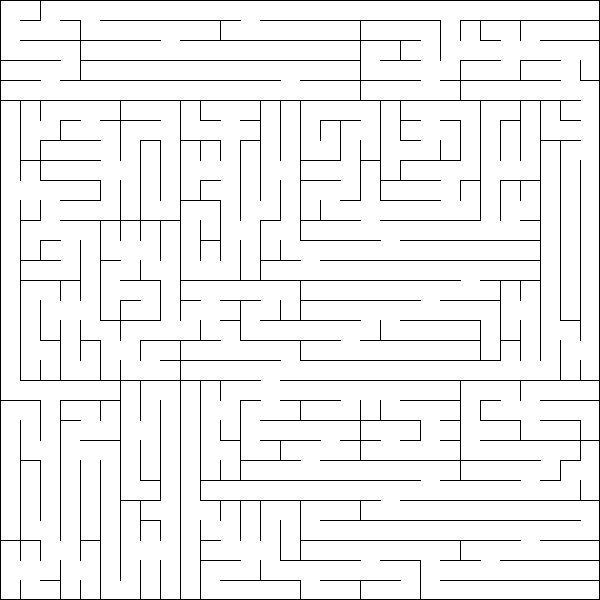
\includegraphics[width=0.8\linewidth]{maze.jpg}
\end{center}
%\vspace{-5.7cm}
\end{minipage}

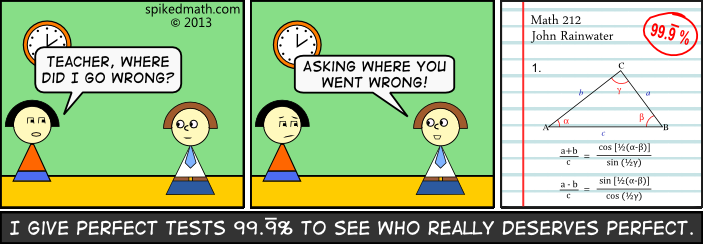
\includegraphics[width=0.9\textwidth]{547-the-perfect-score.png}
\begin{center}
\tiny Mike, http://http://spikedmath.com/547.html, CC-BY-NC-2.5
\end{center}
\end{minipage}

\end{document}
